\chapter{Introdução}
\label{cap:introducao}

Este capítulo apresenta a contextualização do trabalho descrito nesta dissertação, o problema
que motiva a sua realização, as questões de investigação e os objetivos definidos, as
contribuições científicas e a organização do documento. Quem o leia fica a saber que problema o trabalho resolve, para quem, e o que o sistema recusa fazer por decisão e não por limitação.

\section{Contextualização}
\label{sec:intro_origem}

A aquisição de ações tornou-se uma operação de baixa fricção, acessível através de aplicações
móveis e sem custos de corretagem significativos. A maioria dos adultos norte-americanos detém
hoje ações, diretamente ou através de fundos e planos de reforma \autocite{gallup2025stock}, num
mercado cuja capitalização excede os 62 biliões de dólares \autocite{sifma2025factbook}, conforme
representado na Figura~\ref{fig:mercado_eua}.

A facilidade de acesso não se estendeu, contudo, à interpretação da informação. Quando o preço de
um ativo se move, o investidor particular dispõe de instrumentos limitados para determinar o
significado desse movimento.

O comportamento deste segmento é objeto de investigação corrente, e dois resultados recentes
delimitam o problema tratado nesta dissertação. O primeiro é o de que a atenção do investidor
particular constitui hoje uma quantidade medida, cujos indicadores são discutidos e comparados na
literatura \autocite{cahill2025attention}: aquilo que determina o que o investidor observa é
estudado como variável, e não como acaso. O segundo é o de que a participação do investidor
particular no mercado, e as condições em que negoceia, permanecem tema de revisão ativa
\autocite{ernst2026retail}. O Capítulo~\ref{cap:contexto} desenvolve os mecanismos
comportamentais que esta literatura documenta, e que explicam por que razão a ausência de contexto
é mais onerosa para este público do que para um profissional.

Interessa reter deste conjunto o que delimita o problema. Os sinais que captam a atenção do
investidor chegam-lhe sem contexto, e a decisão que se lhes segue é tomada sob condições que a
literatura documenta como desfavoráveis. Três questões concretas permanecem por responder no
momento em que o investidor observa um movimento de preço:

\begin{enumerate}
  \item \textbf{o movimento é invulgar?} Uma variação de quatro por cento representa um
        acontecimento raro numa empresa de baixa volatilidade e um dia comum numa empresa volátil;
  \item \textbf{a origem do movimento é a empresa ou o mercado?} Uma descida que acompanha o
        mercado e uma descida isolada correspondem a situações distintas;
  \item \textbf{existem precedentes, e qual foi o seu desfecho?} A existência de dias comparáveis
        no passado, e do que se lhes seguiu, permite situar o movimento observado.
\end{enumerate}

As aplicações gratuitas correntes apresentam a variação percentual e não respondem a nenhuma
das três. Existem produtos recentes que declaram ir além disso, e a
Secção~\ref{sec:ctx_ferramentas} nomeia-os: o que as respetivas páginas descrevem é um resumo
em linguagem natural, e não os casos passados individualizados com o desfecho medido. Os
terminais de informação financeira profissional respondem às três, e não estão disponíveis em
regime gratuito nem acessível ao perfil de investidor em causa. A lacuna não decorre da indisponibilidade de
dados, que existem em quantidade e são gratuitos, mas da ausência de contexto verificável
construído sobre eles.

A Figura~\ref{fig:intro_lacuna} apresenta a diferença sobre um acontecimento concreto.

\begin{figure}[htbp]
\centering
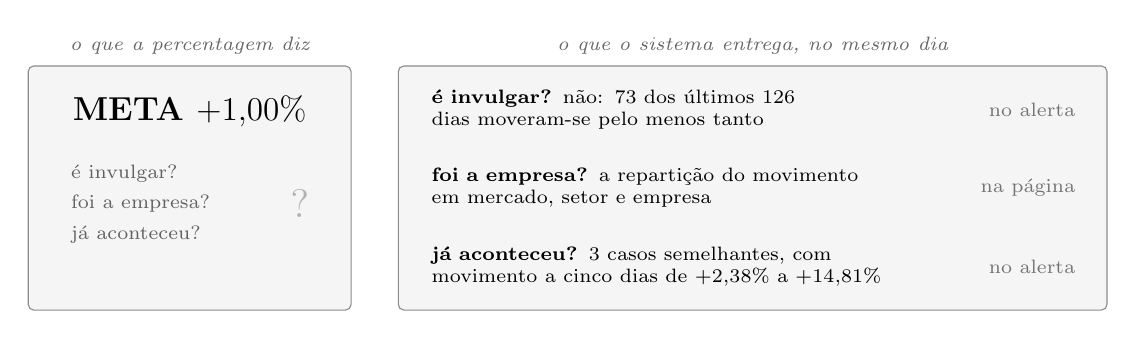
\begin{tikzpicture}[font=\footnotesize,
  cx/.style={draw=black!45, rounded corners=2pt, inner sep=0pt},
  tit/.style={font=\scriptsize\itshape, text=black!60},
  q/.style={font=\scriptsize, align=left, anchor=west, text width=6.35cm},
  onde/.style={font=\scriptsize, text=black!55, anchor=east},
]
  % caixa da esquerda: de 0,00 a 4,10 · caixa da direita: de 4,70 a 13,70
  \node[cx, fill=black!4, minimum width=4.1cm, minimum height=3.1cm] at (2.05,1.35) {};
  \node[cx, fill=black!4, minimum width=9.0cm, minimum height=3.1cm] at (9.2,1.35) {};

  \node[tit] at (2.05,3.16) {o que a percentagem diz};
  \node[tit] at (9.2,3.16) {o que o sistema entrega, no mesmo dia};

  \node[font=\large\bfseries] at (2.05,2.32) {META $+1{,}00\%$};
  \node[font=\scriptsize, align=left, text=black!62, anchor=west] at (0.42,1.15)
       {é invulgar?\\[3pt] foi a empresa?\\[3pt] já aconteceu?};
  \node[font=\Large, text=black!30] at (3.45,1.15) {?};

  \node[q] at (5.00,2.35)
       {\textbf{é invulgar?} não: $73$ dos últimos $126$\\ dias moveram-se pelo menos tanto};
  \node[q] at (5.00,1.35)
       {\textbf{foi a empresa?} a repartição do movimento\\ em mercado, setor e empresa};
  \node[q] at (5.00,0.35)
       {\textbf{já aconteceu?} $3$ casos semelhantes, com\\ movimento a cinco dias de $+2{,}38\%$ a $+14{,}81\%$};
  \node[onde] at (13.42,2.35) {no alerta};
  \node[onde] at (13.42,1.35) {na página};
  \node[onde] at (13.42,0.35) {no alerta};
\end{tikzpicture}
\caption[O mesmo acontecimento, com e sem contexto]{O mesmo dia da mesma empresa, à esquerda
como uma cotação o apresenta e à direita como o sistema o entrega. Os valores da direita são
reproduzidos do alerta enviado ao canal a 8 de setembro de 2026, e não construídos para o
efeito. A terceira coluna indica onde vive cada resposta, e a distinção não é acessória: o
alerta responde à primeira e à terceira perguntas no momento em que interrompe o leitor, ao
passo que a repartição depende do fecho do dia e por isso é apresentada na aplicação, como
mostra a Figura~\ref{fig:sis_empresa}.}
\label{fig:intro_lacuna}
\end{figure}


\begin{figure}[htbp]
\centering
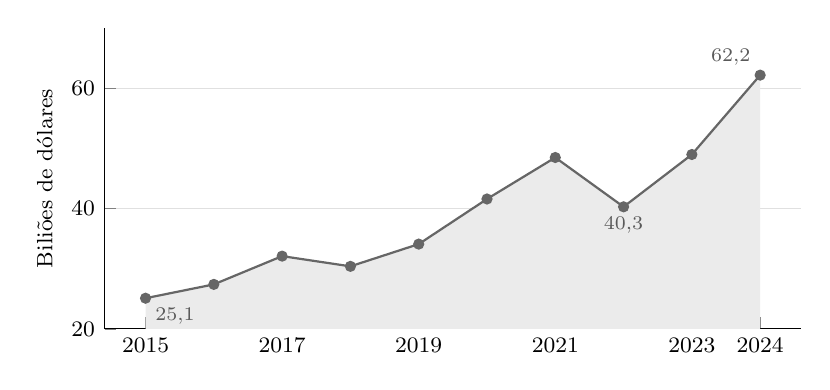
\begin{tikzpicture}
\begin{axis}[
  % Serie temporal: a forma e' a linha, nao a barra. Dez barras rotuladas uma a uma
  % competiam com a leitura que interessa, que e' a trajectoria e a quebra de 2022.
  width=0.86\textwidth, height=5.4cm,
  ymin=20, ymax=70, xmin=2014.4, xmax=2024.6,
  xtick={2015,2017,2019,2021,2023,2024},
  % anos NAO levam separador de milhares: sem isto o pgfplots escreve 2,015.
  xticklabel style={/pgf/number format/.cd, fixed, 1000 sep={}},
  ylabel={Biliões de dólares},
  tick label style={font=\footnotesize}, label style={font=\footnotesize},
  ymajorgrids, grid style={black!12}, axis lines*=left,
  ]
  \addplot[draw=none, fill=black!8, forget plot] coordinates {
    (2015,20) (2015,25.1) (2016,27.4) (2017,32.1) (2018,30.4) (2019,34.1)
    (2020,41.6) (2021,48.5) (2022,40.3) (2023,49.0) (2024,62.2) (2024,20)} \closedcycle;
  \addplot[black!60, thick, mark=*, mark size=1.6pt,
           mark options={fill=black!60, draw=none}] coordinates {
    (2015,25.1) (2016,27.4) (2017,32.1) (2018,30.4) (2019,34.1)
    (2020,41.6) (2021,48.5) (2022,40.3) (2023,49.0) (2024,62.2)};
  % so os tres pontos que a prosa invoca: inicio, a quebra, e o fim.
  \node[font=\scriptsize, black!65, below right] at (axis cs:2015,25.1) {25,1};
  \node[font=\scriptsize, black!65, below] at (axis cs:2022,40.3) {40,3};
  \node[font=\scriptsize, black!65, above left] at (axis cs:2024,62.2) {62,2};
\end{axis}
\end{tikzpicture}
\caption[Capitalização do mercado acionista dos EUA]{Capitalização do mercado acionista dos
Estados Unidos, 2015--2024, em biliões de dólares. Elaborado a partir dos dados do SIFMA Capital
Markets Fact Book \autocite{sifma2025factbook}.}
\label{fig:mercado_eua}
\end{figure}

\section{Descrição do problema}
\label{sec:intro_sistema}

Esta dissertação apresenta o InvestiGator, um sistema de alertas financeiros construído
exclusivamente sobre fontes de dados gratuitas, que monitoriza um conjunto de empresas, deteta
acontecimentos que se afastam do comportamento habitual de cada uma e emite alertas acompanhados
da explicação e da evidência que os sustentam.

O sistema dispõe de dois gatilhos, representados na Figura~\ref{fig:conceito}: um movimento de
preço invulgar para a empresa em causa, ou a chegada de uma notícia relevante sobre ela. Em ambos
os casos, a mensagem entregue identifica o acontecimento, o critério pelo qual foi considerado
invulgar, a proveniência dos dados utilizados e os casos passados semanticamente próximos, com o
comportamento observado do preço após cada um deles.

Uma decisão de desenho atravessa o sistema e condiciona todas as restantes: \textbf{o sistema não
produz previsões de preço}. Não indica direção futura, não emite recomendações de compra ou venda
e não apresenta alvos de preço. Esta restrição tem duas justificações. A primeira é de
verificabilidade: uma afirmação sobre um acontecimento passado pode ser confirmada contra o
registo no momento em que é lida, ao passo que uma previsão só é avaliável depois de a decisão do
investidor já ter sido tomada. A segunda é teórica: a hipótese dos mercados eficientes, na
sua forma semiforte, torna improvável a antecipação sistemática de movimentos a partir de
informação publicamente disponível. O Capítulo~\ref{cap:contexto} desenvolve-a e identifica a
literatura correspondente. Esta dissertação não testa essa hipótese nem se apoia nela para
estabelecer qualquer conclusão.

\begin{figure}[htbp]
\centering
\begin{tikzpicture}[
  font=\small, >={Stealth[length=2.2mm]},
  gat/.style={draw, rounded corners, fill=black!8, align=center, text width=3.1cm, minimum height=1cm},
  sis/.style={draw, rounded corners, fill=black!3, align=center, text width=2.6cm, minimum height=1.6cm},
  saida/.style={draw, rounded corners, fill=black!3, align=center, text width=3.8cm, minimum height=1.6cm},
]
  \node[gat] (g1) {movimento de preço\\ invulgar};
  \node[gat, below=7mm of g1] (g2) {notícia relevante\\ sobre a empresa};
  \node[sis] (sis) at ($(g1)!0.5!(g2) + (3.9,0)$) {\textbf{InvestiGator}};
  \node[saida, right=1.3cm of sis] (out) {alerta explicado\\[2pt]
    \footnotesize o que aconteceu\\ \footnotesize porquê · fontes\\ \footnotesize precedentes};
  \node[right=1.0cm of out, align=center] (inv) {\footnotesize investidor};
  \draw[->] (g1) -- (sis);
  \draw[->] (g2) -- (sis);
  \draw[->] (sis) -- (out);
  \draw[->] (out) -- (inv);
\end{tikzpicture}
\caption[Os dois gatilhos do sistema]{Os dois gatilhos do sistema e a saída que produzem. O
investidor recebe um alerta acompanhado da evidência que permite verificá-lo, e não apenas a
notificação de que o preço se moveu.}
\label{fig:conceito}
\end{figure}

\section{Objetivos e questões de investigação}
\label{sec:intro_objetivos}

O objetivo geral desta dissertação é desenhar, construir e avaliar um sistema de alertas
financeiros explicável para investidores particulares, utilizando exclusivamente fontes de dados
gratuitas.

Deste objetivo decorrem quatro questões de investigação, cada uma associada a uma medição e a um
critério de sucesso definidos antes da execução das experiências:
% A forma longa do acrónimo é dispensada aqui: a frase anterior escreve-a por extenso, e
% `\gls{QI}1` na primeira utilização imprimiria «Questão de Investigação (QI)1», com o
% número colado ao parêntese. O acrónimo continua a constar da Lista de Acrónimos, porque
% as utilizações seguintes de `\gls` continuam a registá-lo.
\glsunset{QI}
\begin{itemize}
  \item \textbf{\gls{QI}1, deteção.} Consegue um método estatístico simples e transparente detetar
        movimentos invulgares de forma consistente entre empresas com volatilidades distintas, e
        fazê-lo melhor do que uma regra de limiar fixo?
  \item \textbf{\gls{QI}2, precedentes.} Consegue o sistema recuperar notícias de outra
        empresa do mesmo setor melhor do que as alternativas textuais e de ordenação avaliadas,
        e conservar vantagem sobre o acaso quando se exigem notícias anteriores à consulta?
  \item \textbf{\gls{QI}3, triagem.} Consegue um modelo treinado decidir que notícias justificam um
        alerta melhor do que uma linha de base baseada apenas em volatilidade?
  \item \textbf{\gls{QI}4, comparabilidade.} Consegue o ajuste contrastivo do codificador,
        treinado para aproximar notícias cuja \emph{magnitude} de movimento subsequente é
        semelhante, melhorar a comparabilidade de materialidade dos precedentes recuperados sem
        custo na relevância temática?
\end{itemize}

A quarta questão exige uma justificação, porque toca a restrição fundadora deste trabalho. O
sistema não prevê, e treinar um codificador sobre desfechos observados poderia parecer contrariar
essa restrição. A distinção decisiva é entre \emph{direção} e \emph{magnitude}: o que a restrição
proíbe é afirmar para onde o preço vai, e o objetivo de treino desta questão é a magnitude do
movimento, tomada em valor absoluto. O que um codificador assim ajustado produz não é uma
afirmação sobre a notícia em análise, mas uma organização da base de casos que aproxima notícias
de materialidade comparável. Para que a distinção seja verificável e não apenas declarada, a
experiência inclui um segundo braço, treinado sobre o retorno \emph{com sinal}: se a direção fosse
tão aprendível como a magnitude, os dois braços seriam indistinguíveis e o argumento cairia.

A segunda questão do investidor, relativa à separação entre a componente de mercado e a componente
específica da empresa, é tratada por uma técnica descrita no Capítulo~\ref{cap:metodologia} mas não
dá origem a uma questão de investigação. A razão é metodológica: a repartição de um movimento não
possui um valor de referência observável contra o qual possa ser comparada, uma vez que essa
quantidade existe apenas relativamente a um modelo. A Secção~\ref{sec:av_decomposicao} estabelece
o que, apesar disso, permanece mensurável nessa técnica.

Estas questões concretizam-se em quatro objetivos:

\begin{enumerate}
  \item construir o sistema completo, desde a aquisição de dados até à entrega do alerta;
  \item avaliar os componentes, com linhas de base transparentes para deteção, recuperação e triagem;
  \item garantir que as explicações apresentadas são fiéis ao que o sistema calculou;
  \item reportar os resultados obtidos, incluindo os que não confirmem as expectativas iniciais.
\end{enumerate}

As técnicas que estes objetivos exigem pertencem a famílias distintas, e a questão de onde se
situa a aprendizagem automática no trabalho tem resposta diferente para cada uma das cinco
decisões que o sistema toma antes de um alerta chegar a alguém. Uma delas é uma regra sem
parâmetros estimados. Uma não utiliza parâmetros além da média e do desvio da janela anterior.
Uma tem os parâmetros estimados por regressão, com encolhimento. Uma recorre a um modelo
pré-treinado por outros e utilizado sem ajuste. Apenas a última tem parâmetros estimados neste
trabalho, sobre o conjunto histórico. O rótulo de inteligência artificial confunde estas
situações, e a Secção~\ref{sec:met_onde_ia} separa-as decisão a decisão, com a aprendizagem que
cada uma exigiria.

\section{Contribuições científicas}
\label{sec:intro_contribuicoes}

Tratando-se de uma dissertação em Engenharia de \gls{IA}, a contribuição não reside na formulação
de um algoritmo novo, mas na seleção, integração e avaliação crítica de técnicas estabelecidas até
constituírem um sistema funcional, explicável e reprodutível. Identificam-se cinco contribuições:

\begin{enumerate}
  \item \textbf{Um sistema completo em funcionamento}, com os dois gatilhos, assente em fontes
        gratuitas e efetivamente implantado, e não uma demonstração laboratorial.
  \item \textbf{Um método reprodutível para medir o comportamento do preço na sequência de
        notícias semanticamente próximas}, combinando recuperação por semelhança de frases com
        janelas de estudo de evento, sem utilização de informação posterior ao momento da decisão.
        O Capítulo~\ref{cap:contexto} identifica as duas linhas de trabalho de que provêm.
  \item \textbf{Um conjunto de dados próprio e um modelo treinado sobre ele}, com 79\,753 exemplos
        construídos a partir do corpus público \gls{FNSPID} \autocite{dong2024fnspid} e de séries
        de preços, com o modelo, a calibração e as métricas conservados como artefactos
        versionados.
  \item \textbf{Uma avaliação dos componentes, com linhas de base para três das quatro técnicas}, incluindo o
        resultado que contraria a hipótese inicial, reportado como tal.
  \item \textbf{Um resultado negativo sobre a aprendizagem de materialidade a partir do texto},
        obtido com um protocolo fixado antes da execução e com um diagnóstico que rejeita
        representações degeneradas antes de qualquer métrica ser interpretada. A primeira
        tentativa produziu exatamente essa degeneração, e o diagnóstico apanhou-a; o
        Capítulo~\ref{cap:avaliacao} reporta as duas.
\end{enumerate}

\section{Estrutura do documento}
\label{sec:intro_estrutura}

O Capítulo~\ref{cap:contexto} apresenta o estado da arte, caracterizando o público-alvo, as
ferramentas atualmente disponíveis e as áreas técnicas de onde provêm os componentes utilizados.
O Capítulo~\ref{cap:metodologia} descreve os dados e as quatro técnicas que constituem o sistema.
O Capítulo~\ref{cap:sistema} descreve a arquitetura do InvestiGator e o percurso de uma notícia
desde a recolha até à entrega. O Capítulo~\ref{cap:avaliacao} apresenta o desenho experimental e
os resultados obtidos para cada questão de investigação. O Capítulo~\ref{cap:conclusoes} sintetiza
as respostas, identifica as limitações do trabalho e enuncia as linhas de desenvolvimento futuro.

Cada mecanismo descrito é ilustrado sobre um caso real, com os valores efetivamente calculados
pelo sistema, e não sobre exemplos construídos para o efeito. Uma das doze empresas, a AMD,
reaparece em três papéis distintos ao longo do documento, e serve de fio a quem quiser seguir
um nome só: é o movimento que a Secção~\ref{sec:met_decomposicao} reparte nas suas três
parcelas, é a empresa que a porta de decisão deixava passar em todas as avaliações
registadas, e é uma das que o modelo pontua sem nunca as ter observado no treino. São três
momentos da mesma empresa e não do mesmo acontecimento.

Duas categorias de material aparecem em inglês, e enunciam-se aqui para que não sejam lidas
como descuido. A primeira são os títulos de notícia citados e os identificadores de empresa,
que provêm de fontes em inglês e são reproduzidos sem tradução: traduzi-los quebraria a
correspondência com o material que o leitor pode consultar, que é a propriedade que este
trabalho existe para preservar. A segunda são as capturas da aplicação, cuja interface é
redigida em inglês por decisão de produto, pela razão que a Secção~\ref{sec:sis_explicacao}
desenvolve; uma captura traduzida mostraria um ecrã que não existe. Tudo o resto, incluindo o
texto desenhado no interior das figuras, está em português.
